\section{Installation Coordination and Support}
\label{sec:fdsp-coord-install}
%						15 pages

%%%%%%%%%%%%%%%%%%%%%%%%%%%%%%%%
%\subsection{Organization}
%\label{sec:fdsp-coord-org}

Installation Coordination and Support %or 
(also called simply \textit{Installation}) is
responsible for coordinating the detector installations, providing
detector installation support and providing installation-related
infrastructure. The installation group management responsibility is
shared by a scientific lead and a technical lead that report to the
Technical Coordinator. The %underground 
group responsible for activities in the underground areas is referred to as
the \dword{uit}. The \dword{itf} group, which delivers equipment to the
Ross Shaft, and the \dword{uit}, which receives the equipment
underground, need to be in close communication and work closely
together.

Underground installation is in general responsible for coordinating
and supporting the installation of the \dwords{detmodule} and providing
necessary infrastructure for installation of the experiment. While the
individual consortia are responsible for the installation of their own
detector equipment, it is essential that the detector installation be
planned as a whole and that a single group coordinates the
installation and adapts the plans throughout the installation
process. The \dword{uit} has responsibility for overall coordination
of the installations. In conjunction with each consortium the
\dword{uit} makes the installation plan that describes how the
\dwords{detmodule} are to be installed. The installation plan is used to define
the spaces and infrastructure that will be needed to install them.
%detectors. 
The installation plan will also be used to define the
interfaces between the Installation group and the consortium
deliverables.

\subsection{UIT Infrastructure}

The installation scope includes the infrastructure needed to install
the \dword{fd} such as the cleanroom, a small machine shop, special
cranes, scissor lifts, and access equipment.  Additional equipment
required for installation includes: rigging equipment, hand tools,
diagnostic equipment (including oscilloscopes, network analyzers, and
leak detectors), local storage with some critical supplies and some
personal protective equipment (PPE). The \dword{uit} will also provide
trained personnel to operate the installation infrastructure. The
consortia will provide the detector elements and custom tooling and
fixtures as required to install their detector components.
%In the case of the single-phase detector the installation
%group will also provide the detector support system (DSS) which
%supports the detector and is needed to bring equipment into the
%cryostat.

%In addition to the installation specific infrastructure the
%installation group will also be responsible for general detector
%infrastructure like electronics racks, cable trays, power, and if
%needed additional optical fibers in the shafts.

 

%The \dword{dune} production phases are divided into
%production setup and production. Scope that represents a one time
%investment is included in production setup while equipment and
%infrastructure that scales with the number of detectors is included in
%production. With this definition several of the possible work packages
%are empty. For example once the surface logistics facility is setup it
%will be used for all \num{4} detectors so its scope is completely under
%production setup.



%The organization of the full installation scope into
%work packages that are associated with the different phase of the
%project and the lower level WBS divisions are shown in
%Figure~\ref{WP_def}.
%\begin{figure}[!h]
 % \begin{center}
%   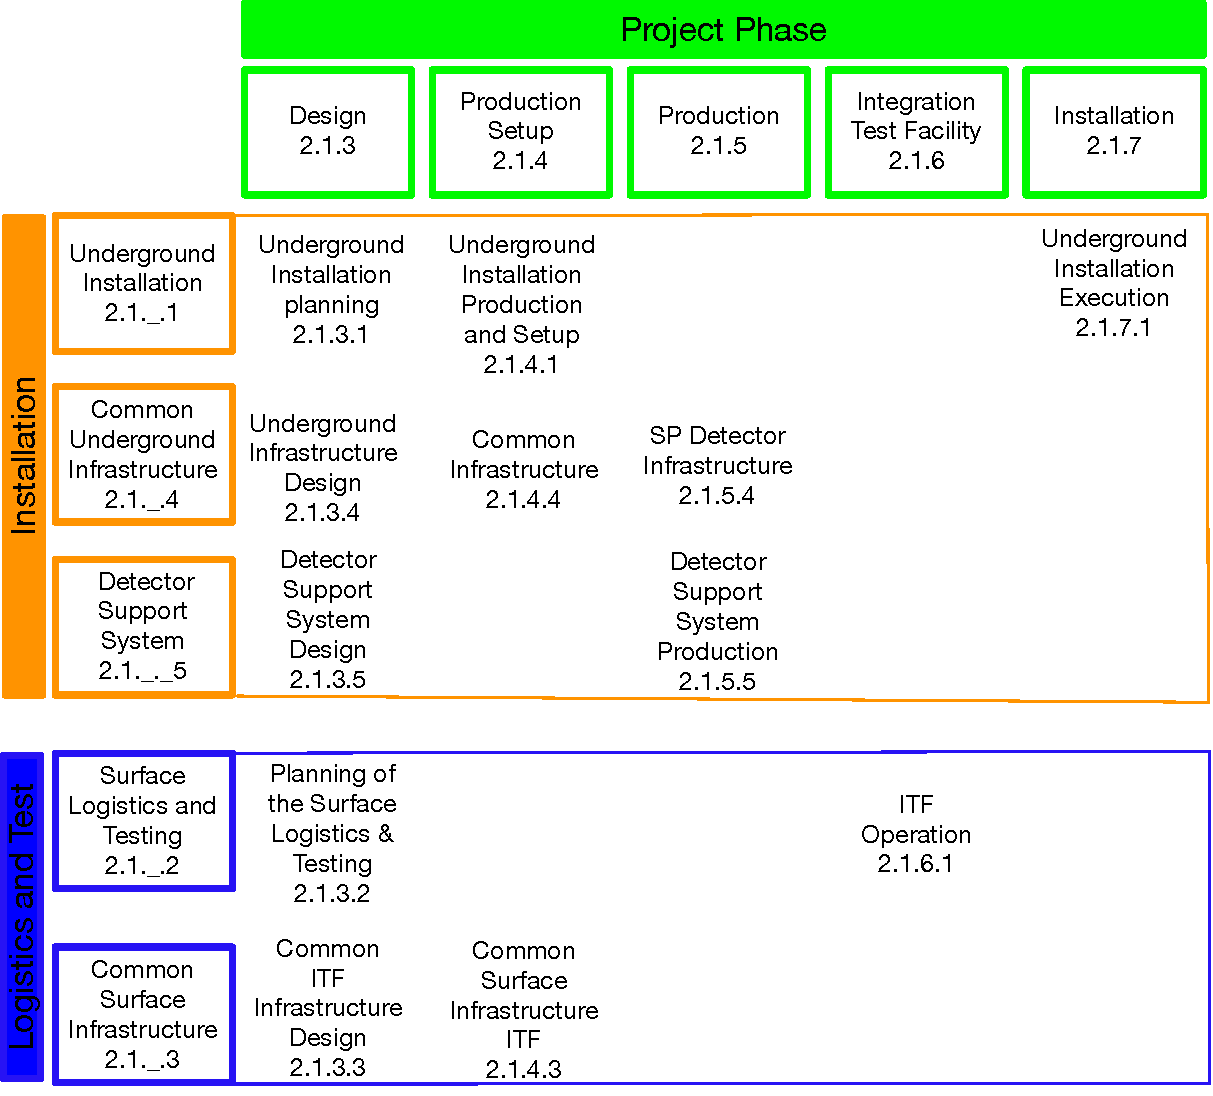
\includegraphics[width=0.8\textwidth]{far-detector-single-phase/figures/OrgChart-v3.pdf}
 %   \caption{Organization of installation and Surface Logistics and
%      Testing. The columns in the matrix represent the project phase
%      and the rows the major divisions in scope. Work packages define
%      the deliverables for each phase according to the major division
%      in scope. }
%    \label{WP_def}
%  \end{center}
%\end{figure}



%%%%%%%%%%%%%%%%%%%%%%%%%%%%%%%%%
\subsection{Surface Logistics \& Testing}
\label{sec:fdsp-coord-integ-test}

The logistics for integrating and installing the DUNE Far Detectors
and their associated infrastructure face a number of
challenges. Possible difficulties include the size and complexity of
the detector itself, the number of sites around the world that will be
fabricating detector and infrastructure components, the necessity for
protecting components from dust, vibration and shock during their
journey to the deep underground laboratory and the lack of space on
the surface near the Sanford Lab Ross Shaft. One mitigation
of these risks is the establishment of a DUNE
Integration and Test Facility (ITF) somewhere in the vicinity of
Sanford Lab. Such a facility and its associated staff would contribute
to DUNE in the following areas.
\begin{itemize}
  \item {\bf Transport Buffer:} Storage capacity for one month
    material in the vicinity of Sanford Lab. Handle packaging
    materials returned from underground laboratory.
  \item {\bf Re-packaging} Facilitate possible re-packaging of
    components before transport underground.
  \item {\bf Component Fabrication:} Possibly provide a capability for
    fabrication of components near Sanford Lab. Undergraduate science
    and engineering students from the South Dakota School of Mines and
    Technology (SDSM\&T) may contribute low cost effort to these
    fabrication activities.
  \item {\bf Component Integration:} Some integration activities may
    be best accomplished in proximity to Sanford Lab. A possible
    example is connecting photodetectors and cold electronics to APAs.
  \item {\bf Inspection, Testing and Repair:} Consortia will define
    their testing requirements including procedures and
    criteria. Consortia will also specify procedures in cases of test
    failure, for example, repair, return to source or discard.
  \item {\bf Visitor Support:} Consortia will likely send staff to the
    ITF for the integration, testing and installation of the consortia
    detector components. The ITF will provide temporary space,
    computer access, assistance personnel and other infrastructure
    support for DUNE visitors.
\item {\bf Outreach:} The ITF may be well located to support a public outreach program. The DUNE Experiment is likely to generate considerable public interest and addressing those interests is important to long-term public support for DUNE specifically and particle physics generally.
\end{itemize}

\subsubsection{Scope}
The scope of the ITF includes several possibly related but mostly
independent tasks. They are:
\begin{itemize}
\item{\bf Cryostat:} The scope of this item is the four cryostats
  planned for installation at the 4850 level of Sanford Lab. Cryostat
  components include the warm steel structure, the stainless steel membrane and
  the insulation. The logistics for the cryostat components will be
  managed by the cryostat installation contractor and LBNF logistics
  coordinator.  Most likely this function will be met with a
  commercial warehousing vendor, who will supply suitable space,
  loading and unloading facilities and a commercial inventory
  management and control system. The vendor will provide all required
  personnel effort as part of its contracted responsibilities.
\item{\bf Cryogenics Systems:} The cryogenics systems are also an LBNF
  responsibility and cryogenics system logistics will likely be
  managed by LBNF similarly to the logistics for the cryostat
  components.
%\item{\bf Cryostat Support Structure:} This structure is an LBNF responsibility and will likely be addressed similarly to the Cryostats and the Cryogenic Systems.
\item{\bf DUNE Detectors:} The DUNE Detectors are the responsibility
  of the Collaboration as implemented by the Consortia. The role of
  the ITF will vary for the several Consortia and a description of
  these various roles is a major topic of this document.
\end{itemize}

\subsubsection{Location }
A reasonable criterion for the location of the ITF is within about an
hour drive from Sanford Lab. That criterion yields the following
possibilities.
\begin{center}
\begin{tabular}{ |c|c| } \hline
{\bf Location} & {\bf 2016 Population}  \\ \hline 
Deadwood & 1,264  \\ 
Lead & 3,010  \\
Rapid City & 74,048  \\
Spearfish & 11,531  \\
Sturgis & 6,832  \\ \hline
\end{tabular}
\end{center}
Since infrastructure is correlated with population, Rapid City would seem the most likely
choice for location with Spearfish as a second possibility. In addition to overall infrastructure,
particular assets of Rapid City include proximity to SDSM\&T and a business community that is
possibly interested in incorporating a DUNE ITF into an overall regional development
program.
%Black Hills State University is located in Spearfish, but that institution is less technology oriented than SDSM\&T.

%$$$$$$$$$$
\subsubsection{\bf Requests from each consortia} 
In February of 2018, questionnaires were distributed to each consortia to seek
their requirements for ITF. Table~\ref{table:leders} lists leaders of each consortia
and names of respondents to the questionnaires, while Tab.~\ref{table:responses}
summarizes their needs for the ITF.
\begin{table}[htbp]
\caption{Leaders and respondents of each consortia.}
\label{table:leders}
\begin{center}
\begin{tabular}{|l|c|c|} \hline
{\bf Consortium} & {\bf Leaders} &{\bf Respondents} \\\hline
High Voltage & Francesco Pietropaolo, Bo Yu & Bo Yu \\ \hline
APA & Stefan Soldner-Rembold, Alberto Marchionni & Peter Sutcliffe \\ \hline
DAQ & Georgia Karagiorgi, Dave Newbold & Alec Habig \\ \hline
SPCE & David Christian, Marco Verzocchi  & Marco Verzocchi, Matt Worcester\\ \hline
DPCE & D. Autiero, T. Hasegawa &  D.Autiero  \\ \hline
SPPD & & \\ \hline
DPPD & Ines Gil Botella, Dominique Duchesneau & Burak Bilki \\ \hline
CISC & &   \\ \hline
CRP & &  \\   \hline
\end{tabular}
\end{center}
\end{table}

\begin{table}[htbp]
\caption{Summary of each consortia's needs at ITF..}
\label{table:responses}
\begin{center}
\scalebox{0.95}
{
\begin{tabular}{|l|c|c|c|c|c|c| } 
\hline
{\bf Consortium} & {\bf Transport} &{\bf Re-Packaging}&{\bf Component}
&{\bf Component}&{\bf Inspection,}&{\bf Visitor} \\
 & {\bf Buffer} &{\bf }&{\bf Fabrication}
&{\bf Integration}&{\bf Testing}&{\bf Support} \\ \hline 
High Voltage & Yes & Yes & No & Yes? & Yes & Yes \\ \hline
APA & Yes & Yes & Yes & Yes & Yes & Yes \\ \hline
DAQ & Yes & Yes & Yes & Yes & Yes & Yes \\ \hline
SPCE & Yes & Yes & No & No & Yes & Yes \\ \hline
DPCE & Yes & No & No & No & Yes & Yes \\ \hline
SPPD & & & & & &  \\ \hline
DPPD & Yes & Yes & Yes & No & Yes & Yes \\ \hline
CISC & & & & & &  \\ \hline
CRP & & & & & &  \\   \hline
\end{tabular}
}
\end{center}
\end{table}

\noindent Responses from each consortia are followed below.

\paragraph{\bf Transport Buffer}
\begin{itemize}
 \item {\bf High Voltage System} $1000~m^2$ maximum needed ($1$ month before the start of 
TPC installation and $1$ month before the end of the TPC installation) in which
$\sim500~m^2$ for dedicated space and  $500~m^2$ for shared space. 
Humidity needs to be $<70\%$. Re-packaging area needs to be class 100,000
and no insects. There also needs to be a crane coverage between buffer and re-packaging areas.
  \item {\bf APA} For 40--80 APAs, say 
minimum of $\sim1000m^2$, including a place for a cleanroom.
This is based on $1$ year APA production 
and assume they will be transported from the manufacturing facility straight after they are made.
The space can be shared.
There need to be crane access, large door openings, height enough to lift boxes and allow fork lift.
 Some APAs will be kept in transport boxes and after the PDs and electronic boxes have been added, 
they will be ``hung'' in a clean, dry area, ready for transport to SURF in a specialized box.
  \item {\bf DAQ} Area for some boxes and crates needed, but not while shipping containers.
And it can be shared..). It should meed standard electronics environment as well.
  \item {\bf Single Phase Cold Electronics} A total of $40~m^2$ of space
to be populated with racks and possibly one cabinet with dry air storage.
The space can be shared, although we would prefer not to have to share the dry air cabinets.
We prefer to avoid storage at temperatures below $10^\circ$C and we would also prefer an environment with a controlled humidity level such that the dew point in the storage area 
is below $5^\circ$C. 

For components that will be installed on the APAs at the integration facility,
they need to be stored (after unpacking) in a dry-air cabinets such that the dew point is 
significantly below that of the room temperature (a relative humidity in the dry air cabinets at the 
level of $30\%$ is sufficient to ensure this). We also need these cabinets to be connected to ground 
such that we can store the components minimizing the possibility of having electrostatic discharge 
damage.
  \item {\bf Dual Phase Cold Electronics} The largest space will be taken by the signal chimneys (box for a chimney $2.2\times0.5\times0.5~m^3$), $240$ chimneys to be installed, $30\%$ buffer.
We would need $50~m^2$ dedicated space out of the total $200~m^2$ space.
No particular environmental requirements are needed, but we would need
handling facilities for the chimneys boxes with weight $\sim100$ kg.
   \item {\bf Dual Phase Photon Detection} We would need a dedicated space of
$45~m^2$ with dark room with climate (temperature and humidity) control.
\end{itemize}

\paragraph{\bf Re-packaging}

\begin{itemize}
  \item {\bf High Voltage System} Nearly all CPA, FC modules are shipped in $20'$ shipping 
containers with high packing density.  These units need to be transferred to the UG crates to be 
provided by the HVS.  During this process, some basic inspection and tests will be performed either 
by HVS personnel or trained ITF staff.  An outer layer of plastic bag/sheet will be removed and 
replaced on the module before mounted into the UG crates.
  \item {\bf APA} We will be using a separate transport box to crane the APAs into the SURF facility, 
therefore will need a crane to repackage in a reasonably clean area. 
  \item {\bf DAQ} We will likely set some stuff up in conjunction with the cold electronics reception/test station.  In which case, that would need to be disassembled and shipped out afterwards.  With respect to the main volume of Production DAQ stuff, it would come in computer boxes, pallets, or possibly electronics racks.  
We are not sure if this would need repackaged to go down the shaft, however.
  \item {\bf Single Phase Cold Electronics} This is hard to predict at this point. For 
examples for detector cables we may want to transfer the cables onto spools that can be used to 
speed up the installation of the cables in the APAs once the APAs are brought into the toaster in the 
mine. For other components (crates, power supplies) we may need to transfer the components from 
the original packing used for the shipment from the institutions where the components were 
fabricated or tested into a different packing that is optimized for the transport in the mine of the set 
of components that are going to be installed in a short time period, or that facilitate lifting the 
components on the top of the cryostat. The possibility of fully populating racks or even crates prior 
to the transport in the mine, installation on the top of the cryostat, cannot be excluded. Depending 
on the nature of the work, we expect that some monitoring or active participation in the 
re-packaging activities will be provided by members of the consortium.
   \item {\bf Dual Phase Cold Electronics} Very likely there will be no re-packaging.
   \item {\bf Dual Phase Photon Detection} The original packaging will be opened for testing of the equipment inside. Re-packaging will be done using the original packaging materials. At this stage, additional external attachments might be added in order to make the package more suitable for underground transportation. These may include vibration dampers, locks, carriage hooks, etc.
\end{itemize}

\paragraph{\bf Component Fabrication} 

\begin{itemize}
  \item {\bf High Voltage System} No need of fabrication capabilities of the ITF.
  \item {\bf APA} There is always a need for technical effort, the specifics of this is difficult to 
evaluate at this time, but may include simple tooling needs, turning, milling, drilling, grinding etc.
  \item {\bf DAQ} We might need for things we didn't anticipate beforehand --- do we need new mounting brackets, strain relief, etc.
  \item {\bf Single Phase Cold Electronics} We do not expect to do any fabrication work at 
the ITF. We cannot however exclude the need for small repairs or the need for the quick fabrication 
of tooling that may be needed either at the ITF or at Sanford Lab. We expect to have engineer(s) and 
technician(s) from the consortium institution available for these activities, but we may need to 
resort to the help of local personnel from the SDSM\&T. For small repairs we are likely to require a 
small electronic shop.
  \item {\bf Dual Phase Cold Electronics} Very likely no need.
  \item {\bf Dual Phase Photon Detection} We might choose to perform the TPB coating of the 
PMTs at ITF. In this case, a coating facility will be established in a dedicated space at ITF, 
dimensions to be determined at a later stage. The operations will be supervised by DPPD and will 
likely be executed by students/engineers. 
\end{itemize}

\paragraph{\bf Component Integration}

\begin{itemize}
  \item {\bf High Voltage System} It is possible that the integration of the top field cage to the 
ground plane (attaching the ground plane tiles to the top FC modules), or the integration of the 
bottom ground plane (linking the ground plane tiles into larger modules) can be carried out at the 
ITF.
  \item {\bf APA} Skilled technical effort will be needed with APA integration assembly, tooling 
attachment, some cabling assistance. Some of this will be because of health and safety reasons. Space requirement is $100 m^2$ for $1$ to $2$ APAs
  \item {\bf DAQ} Possibly, rack stuffing.
  \item {\bf Single Phase Cold Electronics} We expect that the installation and testing of 
the cold electronics onto the APAs that will take place at the Integration facility will be performed by 
member of the Cold Electronics Consortium stationed there. We plan to have a team comprising at 
least one engineer, one technician and several students/postdocs/scientists to perform these 
activities. Students from SDSM\&T could be integrated in this team mostly for the testing activities, 
but we do expect that the majority of the team will be composed by member of the Cold Electronics 
Consortium at all times.
   \item {\bf Dual Phase Cold Electronics} We do not plan to perform integration at the ITF.
   \item {\bf Dual Phase Photon Detection} DPPD deliverables will not require integration with 
other subsystem elements at the ITF.
\end{itemize}

\paragraph{\bf Inspection, Testing and Repair}

\begin{itemize}
  \item {\bf High Voltage System} During the re-packaging of the CPA/FC/GP modules, perform 
visual inspection of damages, electrical continuity test of a set predetermined test points and a 
small number of resistivity measurements.  Test results will be logged in the traveler documents 
accompanying the modules.  Test instruments will be provided by HVS.  Repairs will be performed 
by HVS experts. Entire process needs to be in class $100,000$ clean space. 
  \item {\bf APA} We will need a reasonably clean area for visual inspection and possibly the tension 
of the wires.  And there will be a full test of the APA in a cold box and will require liquid nitrogen.
We might need minor repairs only.
  \item {\bf DAQ} Testing of components to make sure they arrived ok, at the level of ``does it turn on'' or ``there's no link light''.  More detailed testing could be done remotely by DAQ experts and if repairs are needed, it should be shipped back for expert TLC.
  \item {\bf Single Phase Cold Electronics} The Cold Electronics consortium plans to use 
the Integration Facility mostly for installing the Front End Motherboards on the APAs and then 
performing tests of the fully populated APA prior to the shipment of the APA to Sanford Lab. These 
activities will be performed jointly by the APA, Photon Detector and Cold Electronics consortia, 
using equipment that will also be provided by the Cold Instrumentation and Slow Controls 
consortium and by the DAQ Consortium. The facility required for the installation and the test of the 
Front End Motherboards onto the APA should be modeled on the protoDUNE installation area. It 
requires a crane system for lifting the APA from its shipping box, a suspension system using rails 
that can be used to move the APA in and out of an area dedicated to the installation of the 
electronics and in and out of a cold box to be used for tests. Scissor lifts or a system of platforms 
should be in place to allow work at heights. The team responsible for the protoDUNE installation 
should provide feedback in the design of this area. A detailed study of the scheduling for the 
integration of the electronics and the photon detector system on the APA should be done to 
understand how many areas where this work is performed in parallel are needed (we expect that at 
least two stations operating in parallel are requires). At the moment we do not foresee the need to 
perform other tests at the integration facility. We would still prefer to keep the option open for 
having a small laboratory space ($20 m^2$) where we can test Front End Motherboards that do not 
perform as expected after the installation on the APAs to decide whether they should be repaired 
locally or sent back to one of the Consortium institutions for further investigation/repairs.
   \item {\bf Dual Phase Cold Electronics} Just integrity of the transportation packaging, 
no opening of the packaging.
   \item {\bf Dual Phase Photon Detection} We will perform basic operation and quality checks on 
the photodetectors, calibrations systems, cables, fibers and high voltage system components. 
Photodetectors will be tested for basic operation, others might be as simple as visual inspection. 
The laboratory space required for these test is minimum $40~m^2$. This laboratory space must 
have climate control, sufficient electrical and cabling infrastructure (racks, power, lighting, cable 
trays) and reasonable proximity to the DPPD storage area. The testing operations will be supervised 
by DPPD and will likely be executed by students.
\end{itemize}

\paragraph{\bf Visitor Support} 

\begin{itemize}
  \item {\bf High Voltage System} A common shared office space with other consortia member 
would suffice. We expect to have $\sim2$ long term (commute between ITF and SURF),
 up to $5$ short term visitors.
  \item {\bf APA} Likely over a period of 2 years with $4$ people full time plus $4$ people visiting 
part time $50\%$ and $4$ people underground ($1$ engineer, $2$ physicists and $1$ tech) for
 $1$ year.
  \item {\bf DAQ} During commissioning, at least the same size team as will be at Protodune. 
 During operations, probably one or two experts steady-state.
  \item {\bf Single Phase Cold Electronics} We expect that a large
    fraction of the students/postdocs/scientific personnel from the
    consortium will spend long periods of time (between $3$ months and
    $1$ year) at the integration facility and at Sanford Laboratory. A
    smaller fraction of the personnel will commute for shorter periods
    of time. We expect a similar pattern for engineers and
    technicians. Overall, we expect to have a team of 12--15 people
    from the Cold Electronics consortium will be present at all times
    at the Integration Facility. A similar number of people (up to
    $20$) working on the installation of the detector in Sanford Lab
    may also expect to be able to use any support infrastructure for
    visitors at the Integration Facility.
  \item {\bf Dual Phase Cold Electronics} $2$ visitors, stay of the order of a few months.
  \item {\bf Dual Phase Photon Detection} Eight visitors for $4$ months/year; 
four visitors for $12$ months/year.
\end{itemize}

%$$$$$$$$$$

\subsubsection{Management:}
The management of the ITF should likely be provided by one or more
DUNE Collaborating Institutions. A possible choice is SDSM\&T because
of its physical proximity, its understanding of the local
infrastructure and relationships and its ability to provide some
specialized effort and specialized facilities that might benefit
the ITF.  Some preliminary discussions with SDSM\&T management
have already occurred. These discussions should be ongoing as the
parameters for the ITF become more definite.


\subsubsection{Inventory System:}
Effective inventory management will be essential for all aspects of
DUNE detector development, construction, installation and operation.
While its relevance and importance go beyond the Integration and Test
Facility, the ITF is the location at which LBNF, DUNE project
management, consortia scientific personnel and SURF operations will
interface.  We therefore will develop standards and protocols for
inventory management as part of the ITF planning.  A critical
requirement for the project is that the inventory management system
for procurement, construction and installation must be compatible with
future QA, calibration and detector performance database systems.
Experience with past large detector projects, notably NOvA, has
demonstrated that the capability to track component-specific
information is extremely valuable throughout installation, testing,
commissioning and routine operation.  Compatibility between separate
inventory management and physics information systems will be
maintained for effective operation and analysis of DUNE.

DUNE will rely on a commercial vendor for warehouse and logistics
services in Rapid City or another location nearby to SURF.  Warehouse
vendors have a variety of inventory software packages and standards,
and final specification of the DUNE/LBNF system cannot happen until
the project warehouse vendor is selected.  Discussions are being
coordinated closely with LBNF and initial visits and meetings with
warehouse vendors and software suppliers have occurred.  DUNE
scientific personnel will continue to evaluate candidate systems and
assure interoperability with a future physics database
information systems.

Because of the widely distributed nature of the DUNE development and
construction project and the required compatibility with a commercial
warehouse management system, we plan to develop core inventory
management capabilities based on a service-oriented architecture.  URL
connections will be used to pass data (JSON format) to RESTful APIs,
which have task-specific code written in Python that communicates with
standard PostgresSQL database that will be developed for DUNE by
Fermilab.  Specialized code at remote sites would also be in Python.

Implementation within a commercial cloud-based computing environment,
well suited to the international DUNE project, is also under
consideration.  A recent visit to Rapid City revealed that Dakota
Warehouse
(\href{https://dakotawarehouse.com}{https://dakotawarehouse.com}), a
leading candidate for providing LBNF/DUNE warehouse services for
detector components, including cryostat and cryogenic systems, uses a
cloud-based commercial software package, 3PL Central
(\href{https://3plcentral.com}{https://3plcentral.com}), in which
orders of shipments and stock status are entered and queried through
an internet browser interface.  We will consider the feasibility of
this or a similar platform for LBNF and DUNE.


%%%%%%%%%%%%%%%%%%%%%%%%%%%%%%%%
\subsection{Underground Detector Installation}
\label{sec:fdsp-coord-undergd}

For the \dwords{detmodule} to be installed in safe and efficient
manner, the efforts of the individual consortia must be coordinated
such that the installation is planned as a coherent process. The
interfaces between the individual components must be understood
and the spaces required for the installation process planned and
documented. The installation planning must take into account the
plans and scope of the \dword{lbnf} effort and the individual plans of
the nine consortia. By working with the \dword{lbnf} team and the
members of the consortia responsible for building and installing their
components, a joint installation plan and schedule, taking into account
all activities and needs of all stakeholders, can be developed. Although
the organization of the installation effort is still evolving, %the equivalent of the scientific lead is the installation coordinator. 
an installation coordinator will be the equivalent of a scientific lead for this effort.

One of the primary early responsibilities of the \dword{uit} is to
develop and maintain the \dword{dune} installation plan and the
installation schedule. This installation plan 
describes the installation process in sufficient detail to demonstrate
how all the individual consortium installation plans mesh and it 
gives an overview of the installation process. The installation plan
is used by the \dword{uit} to define the underground infrastructure
needed for detector installation and the interfaces it has with respect  to 
the consortia. The \dword{uit} is responsible for reviewing and
approving the consortium installation plans. Approved installation
plans, engineering design notes, signed final drawings, and safety
documentation and procedures are all prerequisites for the \dword{prr}. 
Approved procedures, safety approval, and
proper training are all required before the \dword{uit} performs
work. During the installation phase the installation leadership 
coordinates the \dword{dune} installation effort and adapts the schedule
as needed. The installation coordinator, together with management, will also
resolve issues when problems occur.

The installation infrastructure to be provided by the \dword{uit}
includes: the underground ISO 8 (or class \num{100000}) clean room
used for the installation; cranes and hoists (if they are not
delivered by \dword{lbnf}); and scissor lifts, aerial lifts, and the common
work platforms outside the cryostat. The \dword{uit} will have
responsibility for operating this equipment and assisting the
consortia with activities related to rigging, material transport, and
logistics. Each consortium is responsible for the installation of
their own equipment, so the responsibility of the installation group is
limited, but the material handling scope is substantial. To support
the installation process, an installation floor manager will lead a
trained crew with the main responsibility of transporting the
equipment to the necessary location and operating the cranes, hoists,
and other common equipment needed for the installation. It is expected
that the installation crew will work with the teams from the various
consortia but will mainly act in a supporting function. The
\dword{uit} floor manager will be responsible for supervising the
\dword{uit} crew, but the ultimate responsibility for all detector
components remains with the consortia even while the underground
team is rigging or transporting these components.  This will be
critical in the case where any parts are damaged during transport or installation,
as the consortia need to judge the necessary actions. 
\fixme{judge the situation and determine the necessary actions?}
For this reason,
a representative or point of contact (POC) from the consortia must be
present when any work is performed on their equipment. The consortium
is responsible for certifying that each installation step is properly
performed.

The \dword{uit} acts as the primary point of contact with
\dword{lbnf} and \surf from the time the components reach the Ross
headframe until the equipment reaches the experimental cavern. If
something goes wrong, \surf calls the \dword{uit} leader who then
contacts the responsible party. The consortia are responsible for
delivering to the \dword{uit} all approved procedures and specialized
tooling required for transport. The \dword{uit} leader acts as a point
of contact if the \dword{lbnf} or \surf team has questions or difficulties
with the underground transport.  The \dword{uit} receives the
materials from \dword{lbnf} and \surf at the entrance to the \dword{dune}
excavations. The \dword{uit} then delivers the equipment to the
required underground location.

In an effort to get an early estimate of the equipment required to
install the detectors the \dword{uit} has developed a preliminary
installation plan that outlines the installation process. At present
the installation plan consists of a \threed model of the cryostat in the
excavations. The \dword{spmod} elements are inserted in the
model and a proposal for how they are transported, assembled, and
inserted into the cryostat has been conceptually developed and expressed in a series of images
some of which are shown in Figures~\ref{fig:Install-seq} and~\ref{fig:cpa-fc-unpack-assy}. 
%
Conceptual designs of the infrastructure needed to support
the transport and assembly are also included in the model. See Figures~\ref{fig:Install-ISO-Top} and~\ref{fig:Install-TopView}. With this
as a tool, the proposed installation sequence can be iterated with the
consortia to converge on a baseline installation plan. A similar
process will be followed for the \dword{dpmod} once the base
configuration for the \dword{sp} installation is agreed upon. The
\dword{uit} has focused initially on the \dword{spmod} as the
\dword{sp} components are larger and the installation process more
complex. 

\begin{dunefigure}[APA and CPA installation steps]{fig:Install-seq}
  {Top row from left:  crated \dword{apa} rotating to vertical position;  crated vertical \dword{apa} placed in cart; \dword{apa} panels moved to fixture using the under-bridge crane. Bottom row: series showing \dword{cpa} panels uncrated and moved to fixture. }
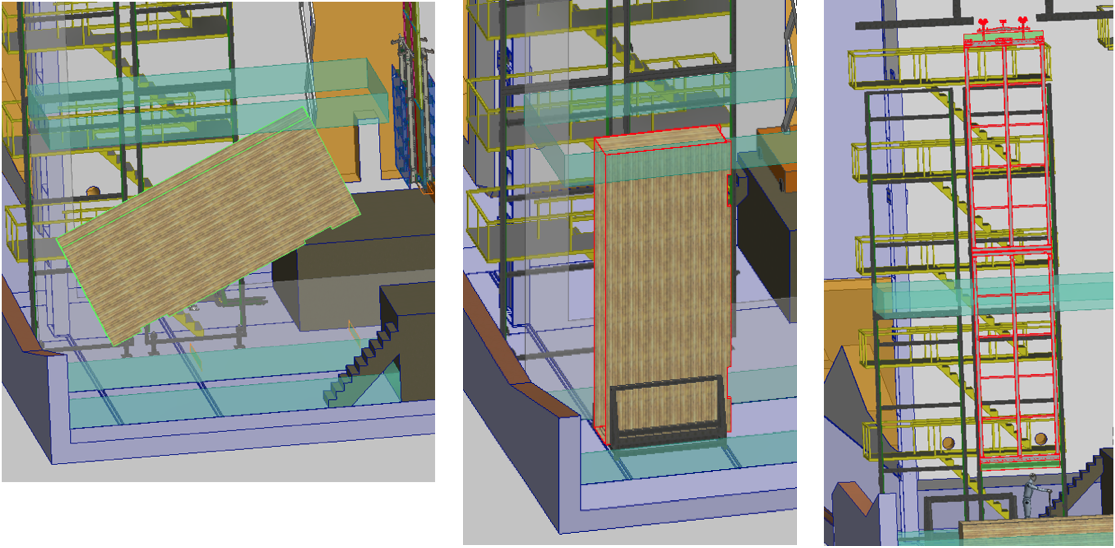
\includegraphics[width=.9\textwidth]{apa-install-seq-top}
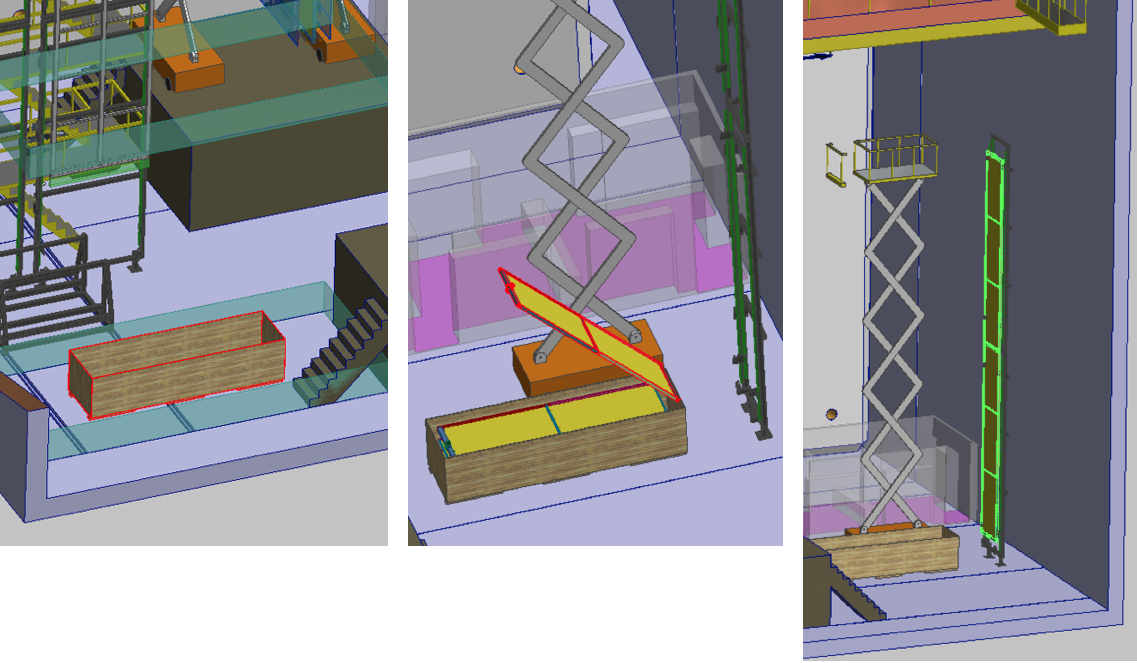
\includegraphics[width=.9\textwidth]{cpa-install-seq-bot}
\end{dunefigure}

\begin{dunefigure}[\dword{cpa} and \dword{fc} unpacking and assembly]{fig:cpa-fc-unpack-assy}
  {On the left, the assembled \dword{cpa} panel is placed onto the north \dword{tco} beam. On the right, the (green) \dword{fc} panels (already lowered into \dword{sas} and moved into the clean room) are installed as the \dword{cpa} array hangs under the \dword{tco} beam. }
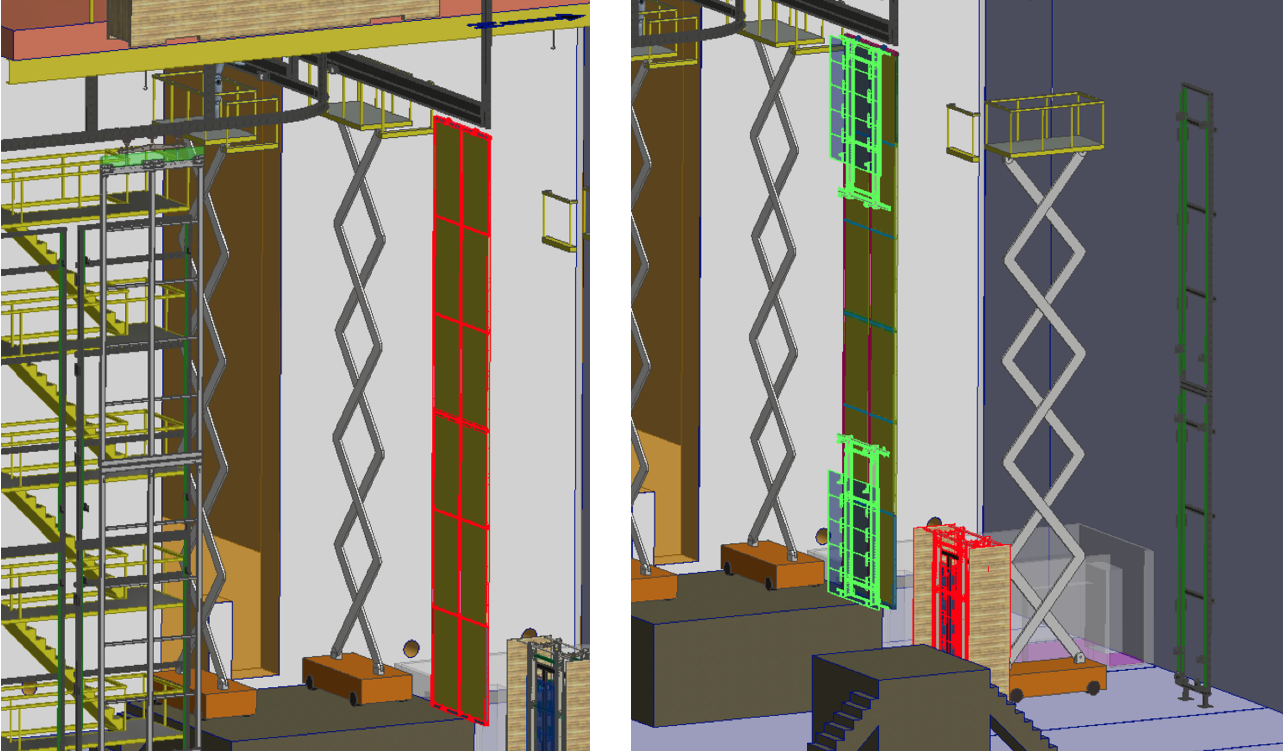
\includegraphics[width=.9\textwidth]{cpa-fc-unpack-assy}
\end{dunefigure}

\begin{dunefigure}[\threed model of underground area showing installation infrastructure]{fig:Install-ISO-Top}
  {\threed model of the underground area showing the infrastructure to install the \dword{spmod} in cryostat~1. The most significant features are presented including the \dword{apa} and \dword{cpa} assembly areas, the region around the \dword{tco} for materials entering the cryostat,  the changing room, the region for the materials air lock, (\dword{sas}), 
  and the means of egress.}
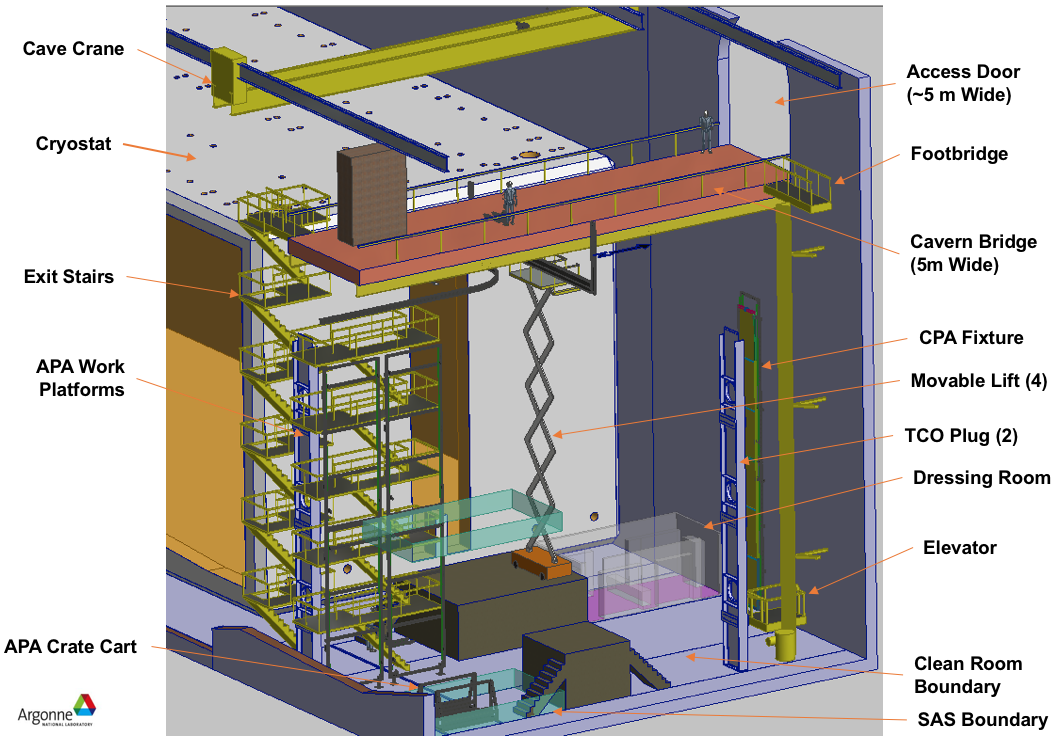
\includegraphics[width=.9\textwidth]{Install-ISO-Top}
\end{dunefigure}

\begin{dunefigure}[Section view of the \threed model showing layout]{fig:Install-TopView}
  {Section view of the \threed model showing layout, looking down on the installation area from below the bridge. Areas shown, left to right,  are the cryostat and \dword{tco}, the platform in front of the \dword{tco}, the dressing area, the \dword{apa} and \dword{cpa} assembly area (directly under the bridge), and the stairs and elevator. The lower right corner of the region is used as the materials air lock.}
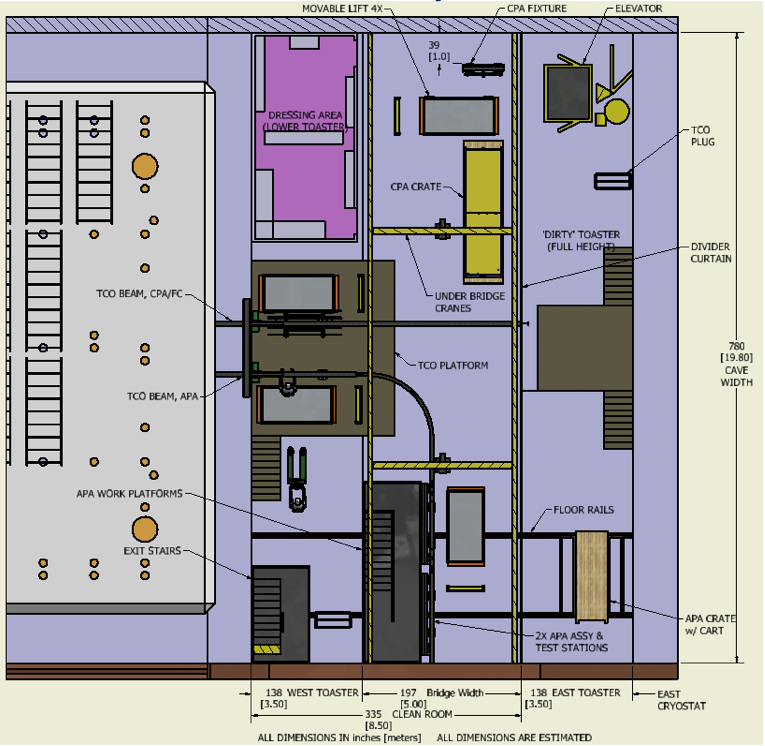
\includegraphics[width=.9\textwidth]{Install-TopView}
\end{dunefigure}





%The current installation plan is described. 
In the current installation plan, \dword{dune} will take
ownership of the different underground areas at different times. The
surface data room and the underground room in the \dword{cuc} are available
significantly before the collaboration has access to the cryostats; 
the optical fibers between the surface and underground will be in
place even earlier. This will allow a \dword{daq} prototype to be developed
and tested early. The installation of the \dword{daq} hardware can also be
finished before the start of detector installation if desired, so the
\dword{daq} will not be on the critical path.  When the collaboration receives
access to Cryostat~1 the steel work for Cryostat~2 will be
finished and the work on installing the membrane will have
started. Excavation will be complete.  For planning purposes it is
assumed that the first \dword{detmodule} will be \dword{sp} and the second
\dword{dp}. The first step in the \dword{sp} installation is to
install the cryogenics piping and the \dword{dss}. As this piping will
require welding and grinding, it is a dirty process and must be
complete before the area can be used as a clean room. When this is
complete the cryostat can be cleaned and the false floor
re-installed. The clean infrastructure for installing the \dword{detmodule},
including the clean room, work platforms, scaffolding, the
fixturing to hold the detector elements during assembly, and all the
lifts need to be set up. Once the infrastructure is in place and the
area is clean, the installation of the main elements can start. The
general layout of the installation area showing the necessary space
and equipment is shown in Figure~\ref{fig:Install-seq}. 

The \dword{spmod}  is installed by first installing the west endwall or
endwall~1 (see Figure~\ref{fig:endwall}).

\begin{dunefigure}[End view of \dword{spmod} with \dword{ewfc} in
  place]{fig:endwall}
  {End view of \dword{spmod} with \dword{ewfc} in
  place, along with one row of \dwords{apa} and \dwords{cpa}.}
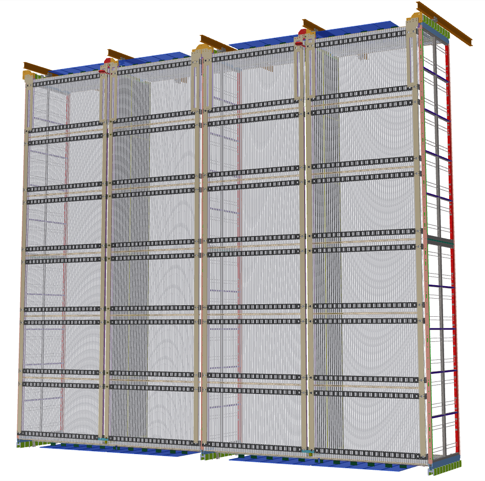
\includegraphics[width=0.6\textwidth]{endwall.png}
\end{dunefigure}

The \dwords{apa} and \dwords{cpa} with top and bottom \dword{fc} panels are
installed next. The plan is to install six \dwords{apa} and four
\dwords{cpa} per week, which is enough to complete one of the \num{25}
rows every week. Additional time is built into the schedule to take
into account that the installation will be slower at the beginning and
some re-work may be needed. By building west-to-east, complete rows can
be finished and tested before moving to the next row. This reduces the
risk of finding a fault after final \dword{fc} deployment and cabling,
which would require dismantling part of the \dword{detmodule}. Some of the steps
needed to install the \dword{apa} and \dword{cpa} modules outside the
cryostat are also shown in Figure~\ref{fig:Install-seq}.  The middle three
panels show how the \dword{apa} needs to be handled in order to rotate
it and mount it to the assembly frame. After two \dwords{apa} are
mounted on top of each other, the cabling for the lower \dwords{apa}, and the
\dword{ce} and \dword{pd} cables can be installed. The
lower three panels show how the \SI{2}{m} \dword{cpa} sub-panels are
removed form the transport crates and assembled on a holding frame. Once
the \dword{cpa} module is assembled the \dword{fc} units can be
mounted. Finally, once the \dwords{apa} and \dwords{cpa} are installed,
the endwall~2 can be installed. A high-level summary of the schedule
is shown in Figure~\ref{fig:Install-Schedule}.

\begin{dunefigure}[High-level installation schedule]{fig:Install-Schedule}
  {High-level installation schedule.}
 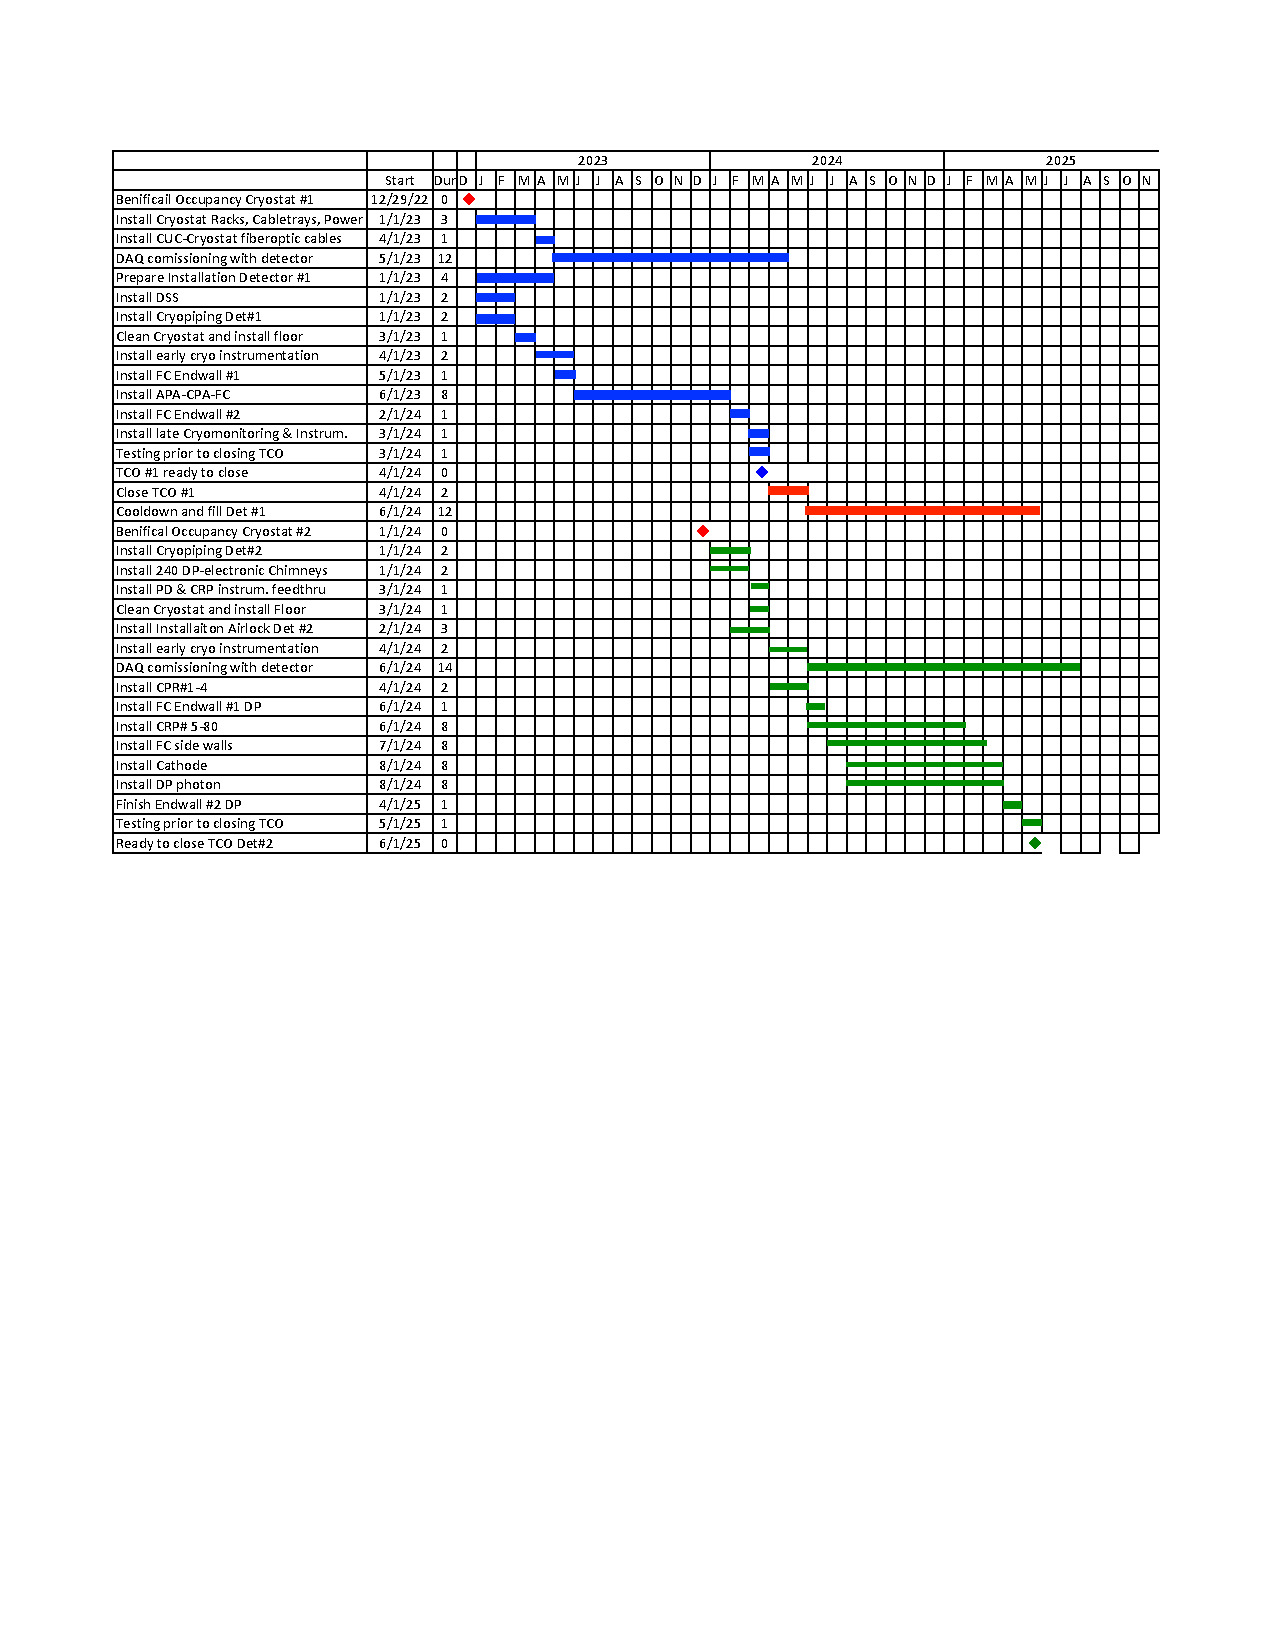
\includegraphics[width=\textwidth]{TP-Schedule-Feb2018.pdf}
\end{dunefigure}


As is seen in the installation schedule the second cryostat becomes
available four months before the first \dword{detmodule} installation is
complete. In this period, installation work for both \dwords{detmodule} 
proceeds in parallel. Like the \dword{spmod}, the first step is
the installation of the cryogenics piping, followed by a thorough cleaning
and installation of the false floor. While this piping is being
installed, the \dword{dp} chimneys for the electronics along with the
\dword{pds} and \dword{crp} instrumentation \fdth{}s can also be installed. Since the
chimneys are installed into the roof of the cryostat,  this work is
performed well away from the final installation work on the first
\dword{detmodule} so there should be no conflicts. Once the first \dword{detmodule} is
installed work on setting up the second \dword{detmodule}'s installation
infrastructure can begin. This work includes moving the cranes and
work platforms along with moving the walls of the clean room so that the
second cryostat is clean. The air filtration to the cryostat is also
moved to the second cryostat.  Since much of the work for the \dword{dp}
installation will be performed inside the cryostat, in principle, outside the cryostat a
clean room area smaller than that for the \dword{spmod}  would suffice. % is needed. 
However, for
planning purposes, it will not be completely clear what type of \dword{detmodule}
will be installed in the second cryostat until fairly late. Therefore the \dword{uit}
will plan to provide a sufficiently large area outside the cryostat to
accommodate either detector technology.  %The \dword{dp} detector itself
%would require 
The much smaller clean room for a \dword{dpmod} %which 
could be installed just
outside the \dword{tco}. The installation process inside the \dword{dpmod} will
proceed east-to-west. At the start of the TPC installation the first
four \dwords{crp} -- comprising the first row -- will be installed. % which comprises the first row of CRP. 
The left panel in Figure~\ref{fig:CRP-Install} shows two \dwords{crp}
being installed near the roof of the cryostat and the right panel
shows one of the \dwords{crp} in a transport box being moved into the cryostat.
Once the first \dword{crp} row is installed and tested, %then 
the first \dword{ewfc} can be installed.%In general rows of \dwords{crp} will be installed and then behind them rows of field cage modules are installed followed by the cathode installation at the bottom of the detector and the photon detector PMTs under the cathode plane. 
In general rows of \dwords{crp} will be installed, followed by rows of \dword{fc} modules, followed by the cathode installation at the bottom of the \dword{detmodule}, followed by 
\dwords{pd} under the cathode plane. 
At the end of the installation, the second \dword{ewfc} is
installed and a final testing period for the full \dword{detmodule} is
foreseen. The \dword{dpmod} installation sequence is shown in green in
Figure~\ref{Install-Schedule}.

\begin{dunefigure}[Image of the \dual CRPs being installed in
  the \dword{dpmod}]{fig:CRP-Install}
  {Left: Image of the \dword{dp} \dwords{crp} being installed in
  the \dword{dpmod}, showing the connection from the \dword{crp} to the
  electronics readout chimney. Right: Image of the \dword{crp} being
  inserted into the cryostat using a transport beam.  The \dual \dword{fc} modules will be inserted in a similar fashion.}
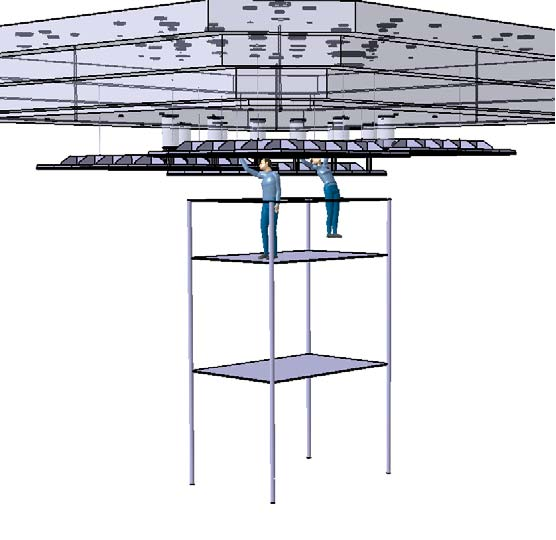
\includegraphics[width=0.45\textwidth]{CRP-install.pdf}
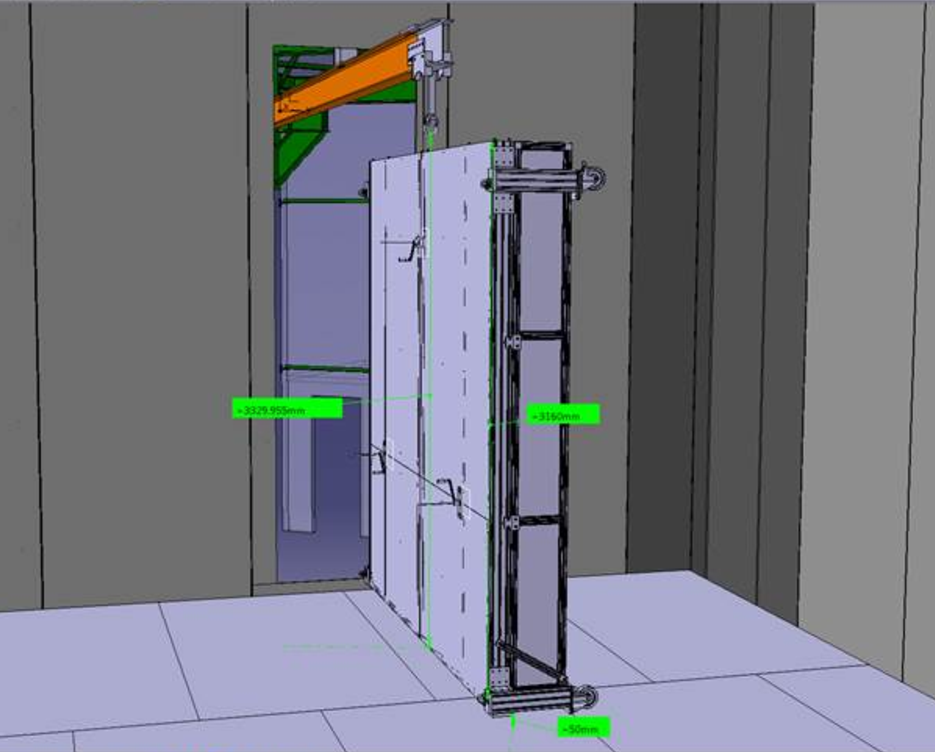
\includegraphics[width=0.45\textwidth]{CRP-into-cryostat.pdf}
\end{dunefigure}

Prior to the \dword{tdr}, mutually agreed upon installation plans must
be approved. These will set the schedule for the installation and will
determine the planning for staffing and budget. Having good estimates
for the time needed and having enough experience to ensure that the
interfaces are understood and the procedures are complete is important
for accurate planning. The experience at \dword{protodune} will be
very important as the \dword{protodune} installation establishes the
procedures for handling all the detector elements and in many cases
gives accurate estimates for the time needed. However, in the case of
the \dword{spmod}, many of these procedures need to revised or
newly developed. For example, the \dword{spmod} will be twice as high as
\dword{pdsp}, so two \dwords{apa} need to be assembled together
and a totally different cabling scheme is needed. Testing the
cabling must be done prior to the \dword{tdr} %as this is needed 
in order to
ensure the design is viable. The \dword{dp} will also need to develop
installation procedures as the \dword{dpmod} 
will have a significantly different \dword{fc} and cathode plane. 

By definition, the installation  is on the critical path, making it vital
that the work be performed efficiently and in a manner that has low
risk. In order to achieve this, a prototype of the installation
equipment for the \dword{spmod}  will be constructed at Ash
River (the \nova neutrino experiment \dword{fd} site in Ash River, Minnesota, USA), and the installation process tested with dummy detector
elements. It is expected that the setup will be available at the time
of the \dword{tdr}, but any lessons learned will need to be implemented and
tested after this. In the period just prior to the start of
installation, the Ash River setup will be used as a training ground for
the \dword{uit}.

%The \dword{uit} is responsible for delivering the common infrastructure
%the detector will need to operate. This infrastructure is typically
%equipment that is used by many groups. This may include: the
%electronics racks with power and cooling, cable trays, the cryostat
%crossing tubes and flanges, rigging equipment, some tools, the ground
%monitoring and isolation transformers, necessary diagnostics equipment
%(including oscilloscopes, a network analyzers and leak detector), a
%small machine shop, storage with some critical supplies, and some PPE.


%\subsection{Detector Support}

The Detector Support System (DSS) provides the structural support for
the single-phase detector inside the cryostat.  It also provides the
necessary infrastructure to move the detector elements into location
during assembly. As the DSS is a new design and is quite different
from the ProtoDUNE DSS it is described in some detail in this
section. The detector elements supported by the DSS include the field
cage endwalls, the \dwords{apa}, and the \dwords{cpa} with top and
bottom field cage panels.  The DSS is supported by the cryostat outer
steel structure through a series of feedthrus which cross through the
cryostat insulation and are anchored with flanges on the cryostat
roof. Inside the cryostat a series of stainless steel I-beams are
connected to the feedthrus and used to support the detector. The DSS
defines the location of the detector inside the cryostat and it also
defines how the detector elements move/contract as the detector is
brought to \dword{lar} temperature. The design of the DSS encompasses
the overall structural design of the detector as only after the
elements are mounted to the DSS and are connected together do they
make a unified mechanical structure. The requirements of the DSS are
as follows:
\begin{itemize}
 \setlength\itemsep{1mm}
\setlength{\parsep}{1mm}
\setlength{\itemsep}{-5mm}
% \small
\item Support the weight of the detector.
\item Accommodate the cryosat roof movement during cryostat filling, testing, and operation.
\item Accommodate variation in the feedthrough locations and
  variation in the flange angles due to installation tolerances and
  loading on the warm structure.
\item Accommodate shrinkage of the detector and DSS from ambient
  temperature to \dword{lar} temperature.
\item Define the position of the detector components relative to each other. 
\item The DSS is electrically connected to the cryostat ground and electrically isolated from the detector.
\item The DSS support penetrations must be purged with GAr to prevent contaminants from diffusing back into the liquid
\item The instrumentation cabling must not interfere with the DSS.
\item The DSS components must be able to be installed through the TCO
\item The DSS is to designed to meet AISC-360 and appropriate codes required by SURF
\item The DSS will be designed to meet seismic requirements 1 mile underground at SURF
\item All materials must be compatible for operation in ultrapure \dword{lar}
\item The DSS beams will be completely submerged in \dword{lar}
\item The DSS will ensure that detector components shall not be less than \SI{400}{mm} from the membrane flat surface
\item The DSS supports shall not interfere with the cryostat I-beam structures
\item The DSS shall be designed such that it supports the detector so that the lower ground plane is above the cryogenic piping and the top of the DSS beams are submerged in \dword{lar} while leaving a 4\% ullage at the top of the cryostat.
\item The DSS shall have infrastructure necessary to move the \dword{apa} and \dword{cpa}-FC assemblies from outside the cryostat through the TCO and to the correct position.
\end{itemize}

Figure~\ref{DSS} (left) shows the DSS structure; there are five rows
of supports for the alternating rows
of \dword{apa}-\dword{cpa}-\dword{apa}-\dword{cpa}-\dword{apa}.  The
DSS is connected to the warm structure at a flange that is mounted on
the outside of the cryostat.  Figure~\ref{DSS} (right) shows the
layout of these structural feedthroughs.  The DSS consists of pairs of
feedthroughs that support \SI{6.4}{m}-long S8x18.4 stainless steel I-beam
sections. The proposed design of the DSS has \num{10} I-beam segments per
row for a total of \num{50} I-beam segments. Each I-beam is suspended on
both ends by rods from feedthroughs that penetrate the roof.  In the
cold condition each beam will shrink which will cause gaps to form
between \dwords{apa} that are adjacent but supported on separate
beams.  \dwords{apa} that are supported on the same beam will not have
gaps develop because both the beam and \dwords{apa} are stainless
steel so they will shrink together.  Each beam is supported by a
nearly \SI{2}{m} long rod that allows the beam support to move as the beam
contracts.
%\fixme{too much detail}
%The feedthrough consists of a flange and $8 ^{''}$ OD structural tube
%welded to it that extends through the cryostat insulation.  There is a
%nominal \SI{10}{mm} gap between the OD of the tube and the ID of the
%clearance tube in the cryostat.  The purpose of the $8 ^{''}$ tube is
%to provide lateral support to the I-beams during installation.
%Running down the center of the feedthrough is a $1^{"}$ diameter rod that
%is supported at a swivel washer at the flange and then supports the
%I-beam at a clevis.  The gas seal is obtained by Conflat Flange and a
%bellows that seals around the swivel washer.  The lateral position of
%the rod can be adjusted to adjust the height of the DSS I-beams.
\begin{figure}[htbp]
\begin{center}
\begin{minipage}[c]{0.49\textwidth}
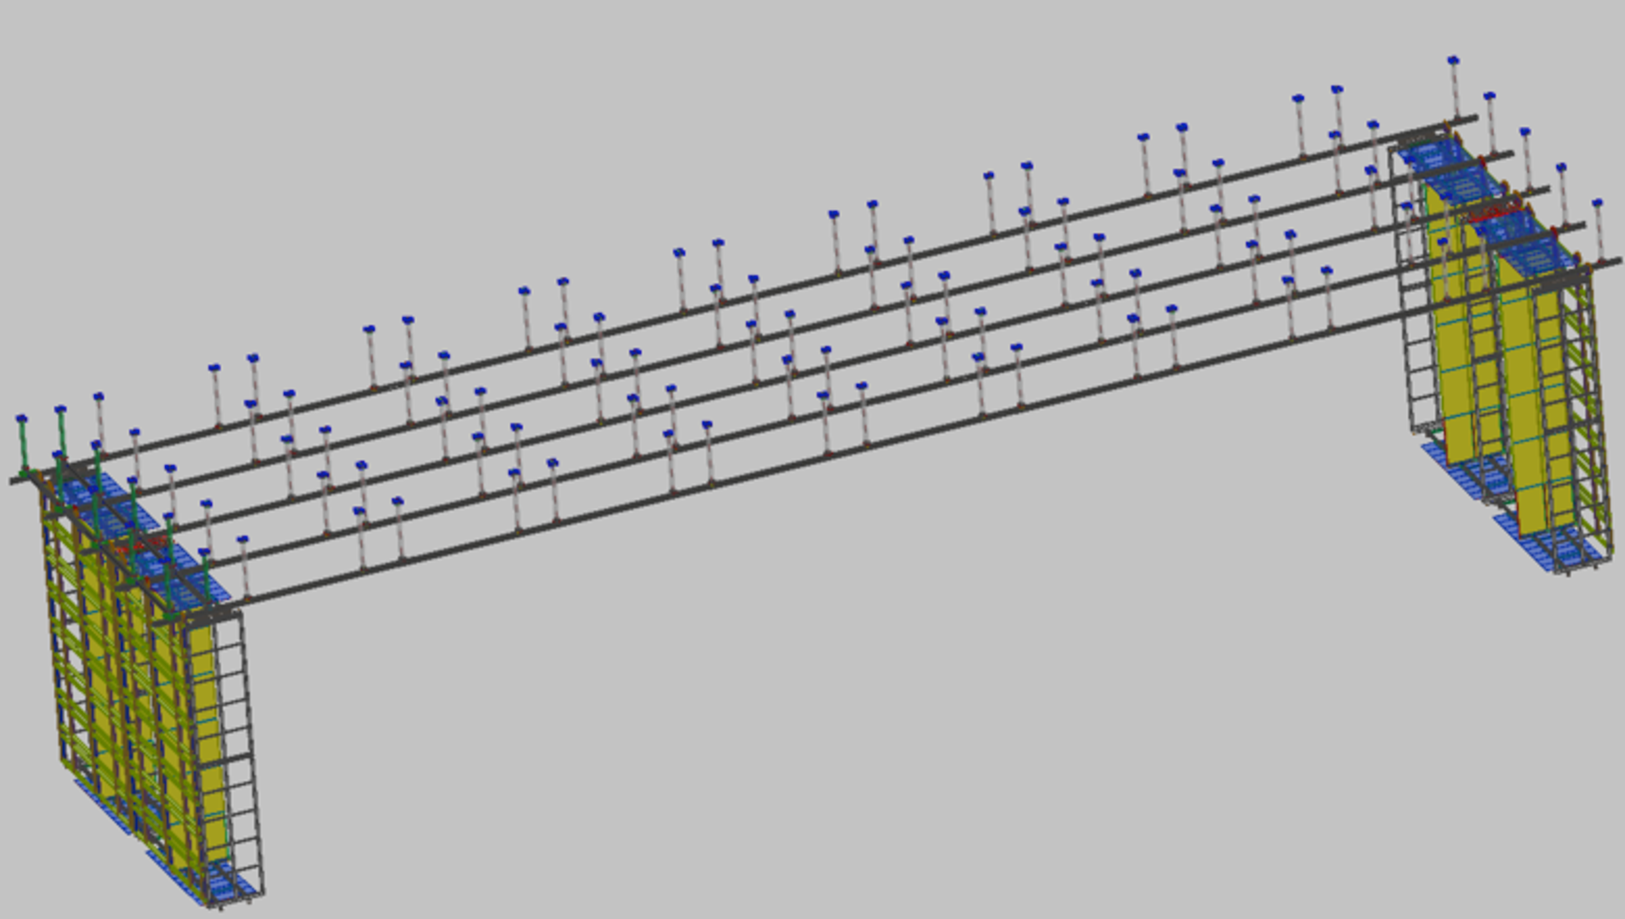
\includegraphics[width=\textwidth]{far-detector-single-phase/figures/DSS-1.pdf}
\end{minipage}
\begin{minipage}[c]{0.49\textwidth}
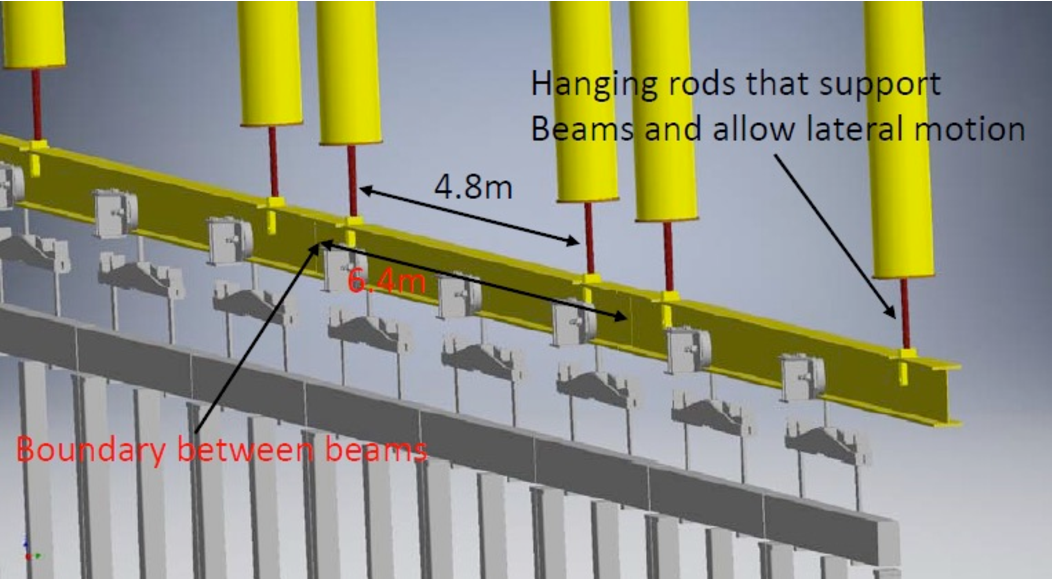
\includegraphics[width=\textwidth]{far-detector-single-phase/figures/DSS-2.pdf}
\end{minipage}
\caption{3-D model of the Detector Support System showing the entire structure on the left along with one row of \dword{apa} and \dword{cpa}/FC at each end. The right panel is a zoomed image showing the connections between the vertical supports and the horizontal I-beams.}
\label{DSS}
\end{center}
\end{figure}


Detector components will be installed using a shuttle beam system
illustrated in Fig.~\ref{shuttle}.  The last two columns of
feedthroughs (eastern most) will support temporary beams that run
north-south, perpendicular to the main DSS beams.  A shuttle beam
%shown in orange
will have trolleys mounted to it and will transverse
north-south until aligned with the required row of DSS beam.  The last
\dword{apa} or \dword{cpa} in a row is supported by the shuttle beam which is bolted
directly to the feedthroughs once it is in place.  As the last \dword{cpa} or
\dword{apa} in each row is installed the north-south beams are removed.

There will be a mechanical interlock system that prevents trolleys
from passing the end of the shuttle beam unless it is aligned with a
corresponding DSS beam.  The shuttle beam and each detector will be
moved using a motorized trolley.  A commercially available motorized
trolley will be modified as needed to meet the needs of the
installation.
\begin{figure}[htbp]
\begin{center}
\begin{minipage}[c]{0.49\textwidth}
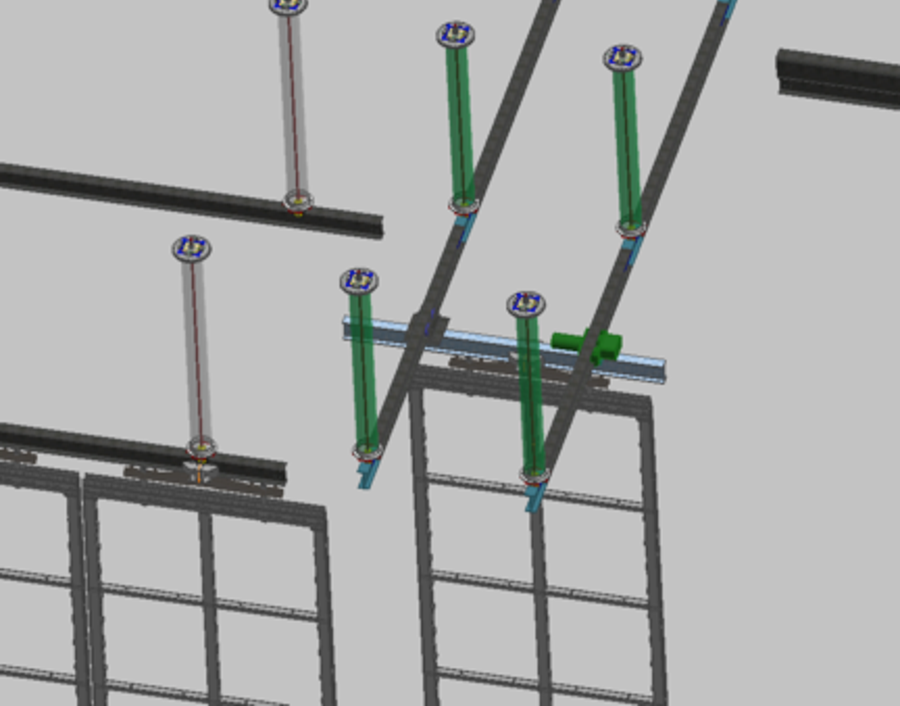
\includegraphics[width=\textwidth]{far-detector-single-phase/figures/Shuttle-1.pdf}
\end{minipage}
\begin{minipage}[c]{0.42\textwidth}
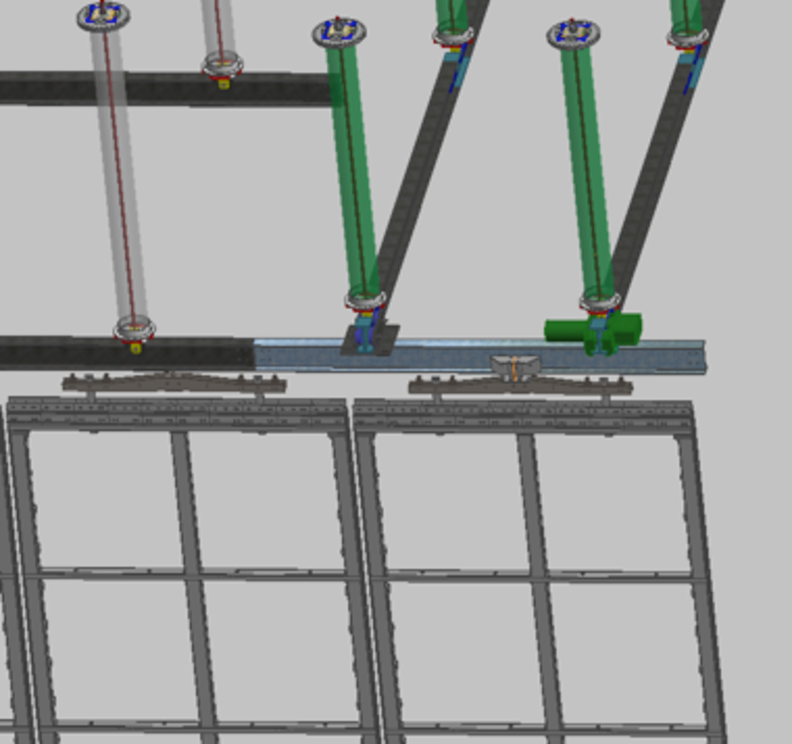
\includegraphics[width=\textwidth]{far-detector-single-phase/figures/shuttle-2.pdf}
\end{minipage}
\caption{3-D models of the shuttle beam end of the DSS. The figures show how an \dword{apa}
is translated into position using he North-South beams until it lines up with the correct
row of I-beams.}
\label{shuttle}
\end{center}
\end{figure}

The DSS installation begins with the placement and alignment of all
the feedthroughs onto the flanges that are mounted to the warm vessel.
There are \num{25} feedthroughs per row and five rows for a total of \num{125}
feedthroughs.  A fixture with a tooling ball will be attached to the
clevis of each feedthrough.  The $XY$ position in the horizontal plane
and the vertical $Z$ position of this tooling ball will be defined.  A
survey will be performed to determine the location of each tooling
ball center and $XY$ and $Z$ adjustments will be made to get the tooling
ball centers to within $\pm$\SI{3}{mm}.  The \SI{6.4}{m} long I-beams will then be
raised and pinned to the clevis.  Each beam weights roughly 350~lbs.
A lifting tripod will be placed over each of the feedthroughs
supporting a beam and a $1/4 ^{''}$ cable will be fed through the top
flange of the feedthrough down the \SI{14}{m} to the cryostat floor where it
will be attached to the I-beam.  The winches on each tripod will raise
the beam in unison in order to get it to the correct height to be
pinned to the feedthrough clevis.  Once the beams are mounted a final
survey of the beams will occur to ensure they are located and aligned
to each other properly.

A mock up of the shuttle system will be constructed to test the
mechanical interlock and drive systems for the shuttle beam
for each detector.  Tests will be conducted to evaluate the level of
misalignment between beams that can be tolerated and the amount of
positional control that can be achieved with the motorized trolley. It
is expected this will be finished prior to the TDR. At the time of the
TDR a larger prototype installation at Ash River will be under
construction. This prototype will use full scale elements and will be
used to develop the installation procedures and to also test the
detector installation process.


\subsection{Preparation for Operations}

After the \dwords{detmodule} are installed in the cryostats there remains a lot
of work before they can be operated. First the \dword{tco}
must be closed. This requires bringing back the cryostat manufacturer. 
First the missing panel with the steel beams
and steel panel are installed to complete the cryostat's outer
structural hull. Then the remaining foam blocks and membrane panels
are installed from the inside using the roof access holes 
to enter the cryostat. 

In parallel, the \lar pumps are installed at
the ends of the cryostat and final connections are made to the
recirculation plant. Once the pumps are installed, the cryostat is
closed, and everything is leak tested, the cryogenics plant can be
brought into operation. First the air inside the cryostat is purged by
injecting pure argon gas at the bottom %of the detector 
at a rate such
that the %detector 
cryostat volume is filled uniformly but faster than the diffusion
rate. This produces a column of argon gas that rises through the volume %detector
and sweeps out the air. This process is referred to as the \textit{piston
purge}. When the piston purge is complete the cool-down of the \dword{detmodule}
can begin. Misting nozzles inject a liquid-gas mix into the cryostat
that cools the detector components at a controlled rate. 

Once the detector is
cold the filling process can begin. Gaseous argon stored at the surface 
at \surf is brought down the shaft and is re-condensed underground. The \lar then flows through filters to remove any H$_2$O or O$_2$ and
flows into the cryostat. Given the very large volume of the cryostats
and the limited cooling power for re-condensing, it is  %the liquid is
expected to take \num{12} months to fill the first \dword{detmodule} and \num{14} months to
fill the second. During this time the detector readout electronics
will be on monitoring the status of the detector. % so the status of the detector can be monitored. 
Once the
\dword{detmodule} is full, the drift high voltage can be carefully ramped up and
data taking can begin.


